\documentclass{article} % Document class declaration
\usepackage{hyperref} % For clickable links
\usepackage{graphicx}
\usepackage{float}

\title{First Homework report} % Title of the document
\author{Andrey Donetskov} % Author name
\date{\today} % Date of compilation


\begin{document} % Start of document content
\maketitle % Generate title
\newpage
In this report, I will discuss two files: \textbf{statistics.ipynb} 
and \textbf{visualization.ipynb}. Both files relate to the 
\textbf{First Mandatory Homework} and cover \textbf{wrecked data}
statistical analysis and corresponding visualizations.

\section{Visual analysis}

Here I trided my best to visualize and clean \cite{data_link}. Below you can see
what it contains:

\begin{table}[ht]
    \centering
    \begin{tabular}{llllll}
        \hline
        & Animal type & Country & Weight kg & Body Length cm & Gender \\
        \hline
        0 & -- & -- & -- & -- & -- \\
        1 & -- & -- & -- & -- & -- \\
        2 & European bison & Poland & 930.000 & 335.0 & male \\
        3 & European bison & Poland & 909.000 & 311.0 & not determined \\
        4 & European bison\texttrademark & Poland & 581.000 & 277.0 & female \\
        $\vdots$ & $\vdots$ & $\vdots$ & $\vdots$ & $\vdots$ & $\vdots$ \\
        1006 & red squirrel & Poland & 0.346 & 20.0 & female \\
        1007 & hedgehog & Germany & 1.000 & 23.0 & female \\
        1008 & hedgehog & Germany & 0.500 & 17.0 & female \\
        1009 & red squirrel & Poland & 0.346 & 20.0 & female \\
        1010 & hedgehog & Hungary & 0.900 & 16.0 & female \\
        \hline
    \end{tabular}
    \caption{Animal observation \textbf{wrecked data} part 1}
    \label{tab:animal_data}
\end{table}

\begin{table}[ht]
    \centering
    \begin{tabular}{llllllllllll}
        \hline
        & Animal code & Latitude & Longitude & Animal name & Observation date & Data compiled by \\
        \hline
        0 & -- & -- & -- & -- & 03.01.2024 & James Johnson \\
        1 & -- & -- & -- & -- & 03.02.2024 & James Johnson \\
        2 & -- & 52.828845 & 23.820144 & Szefu & 01.03.2024 & Anne Anthony \\
        3 & -- & 52.830509 & 23.826849 & -- & 01.03.2024 & Anne Anthony \\
        4 & -- & 52.834109 & 23.807093 & -- & 01.03.2024 & Anne Anthony \\
        $\vdots$ & $\vdots$ & $\vdots$ & $\vdots$ & $\vdots$ & $\vdots$ & $\vdots$ \\
        1006 & -- & 52.212001 & 21.033187 & Lola & 7 May 2024 & Anne Anthony \\
        1007 & -- & 49.561356 & 11.105334 & -- & 7 May 2024 & Bob Bobson \\
        1008 & -- & 49.561569 & 11.087046 & -- & 7 May 2024 & Bob Bobson \\
        1009 & -- & 52.212001 & 21.033187 & Lola & 7 May 2024 & Anne Anthony \\
        1010 & -- & 47.509860 & 18.939943 & -- & 8 May 2024 & Anne Anthony \\
        \hline
    \end{tabular}
    \caption{Animal observation \textbf{wrecked data} part 2}
    \label{tab:animal_data}
\end{table}

Yep. It pretty cursed. I cleaned it:

\begin{enumerate}
  \item Dropped rudimet columns.
  \item Dropped lines with NaNs.
  \item Stardartized objects manually renaming whem.
  \item Multipy negative values by $-1$.
\end{enumerate}

After this I visualized everithing.

\subsection{Count plots}

\begin{figure}[h!]
  \centering
  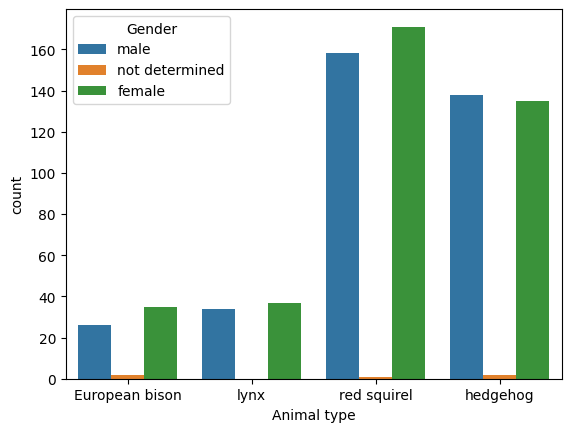
\includegraphics[width=0.45\textwidth]{images/genderplot.png}
  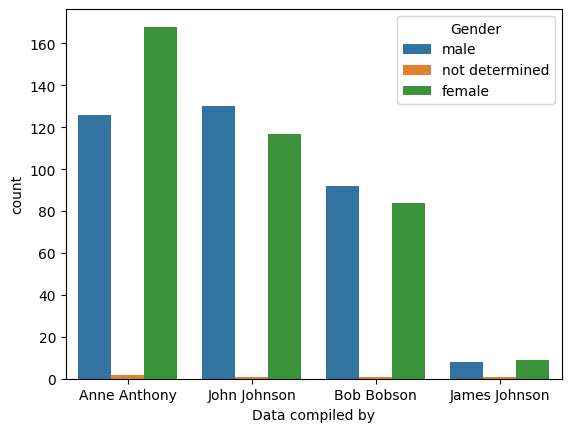
\includegraphics[width=0.45\textwidth]{images/datacompliedbyplot.png}
  \caption{Count plots of animal type and of data contibutor by gender.}
  \label{fig:fig1}
\end{figure}

On~\ref{fig:fig1} gender distribution is normal but anumal type
is not as well as data contibuting. Worth to take a closer look
at James data.

\begin{figure}[h!]
  \centering
  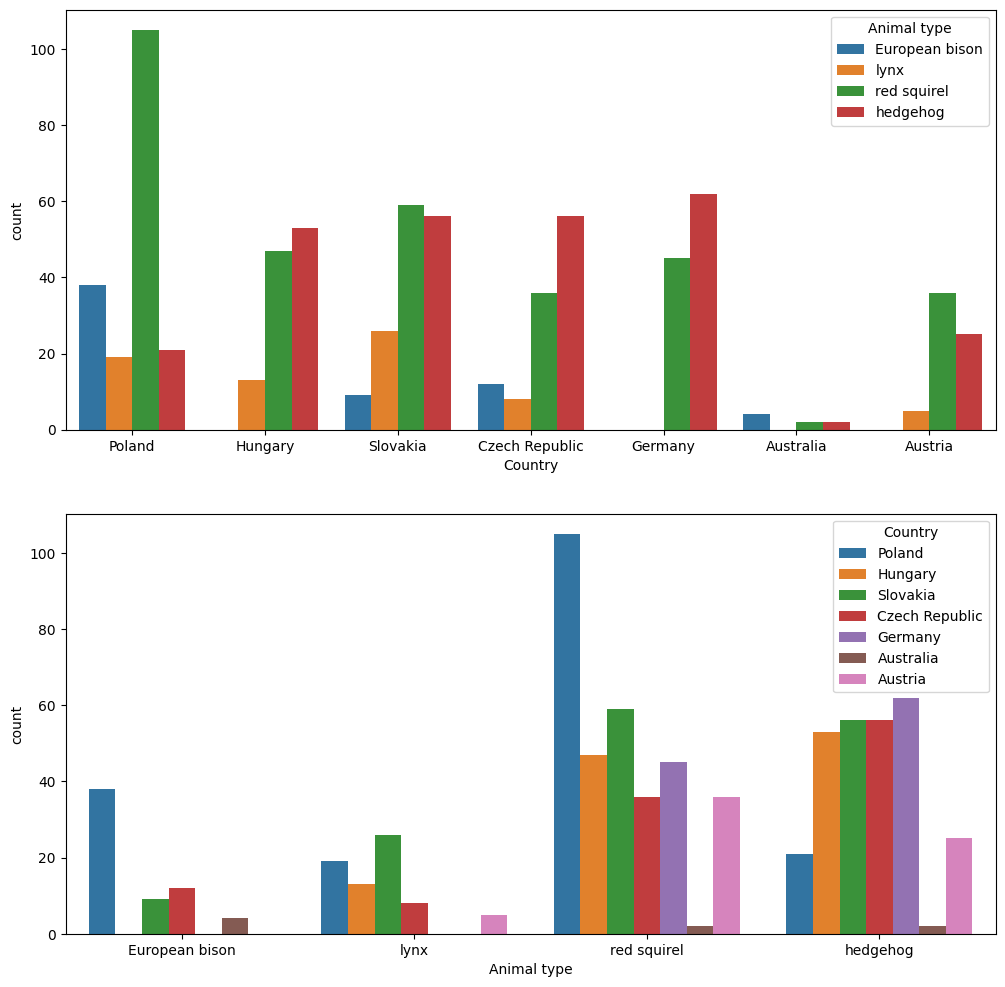
\includegraphics[width=0.65\textwidth]{images/countryanimalcount.png}
  \caption{Count plot of animal type by country and vise versa.}
  \label{fig:fig2}
\end{figure}

On~\ref{fig:fig2} plots I note nothing except that European bison lives in Australia.

\subsection{Line plots}

\begin{figure}[h!]
  \centering
  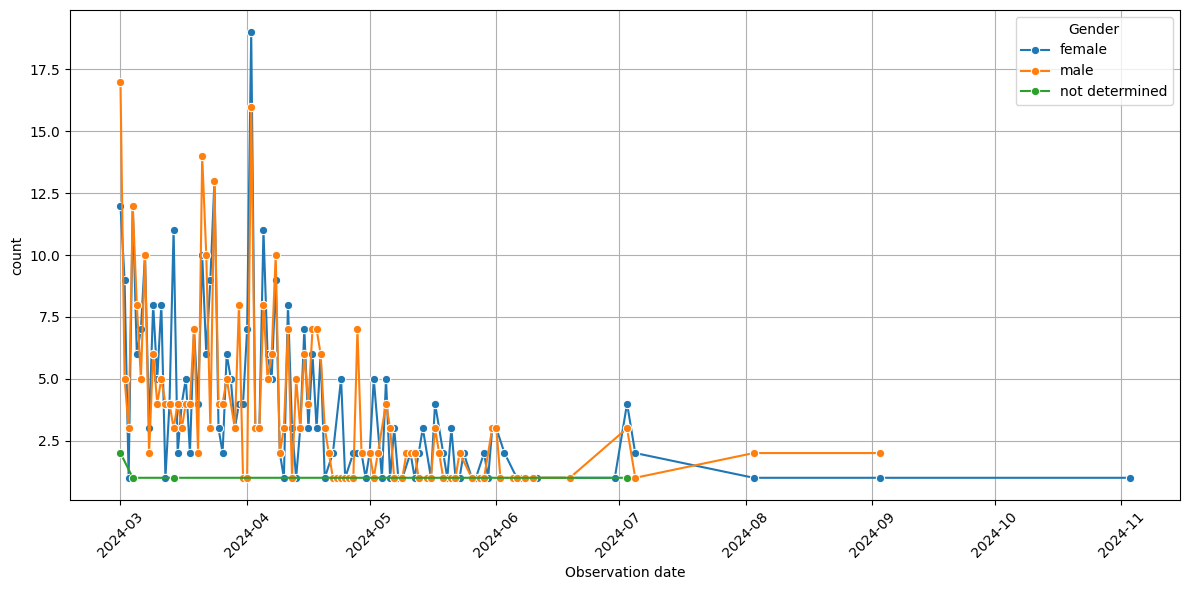
\includegraphics[width=0.8\textwidth]{images/obsdategender.png}
  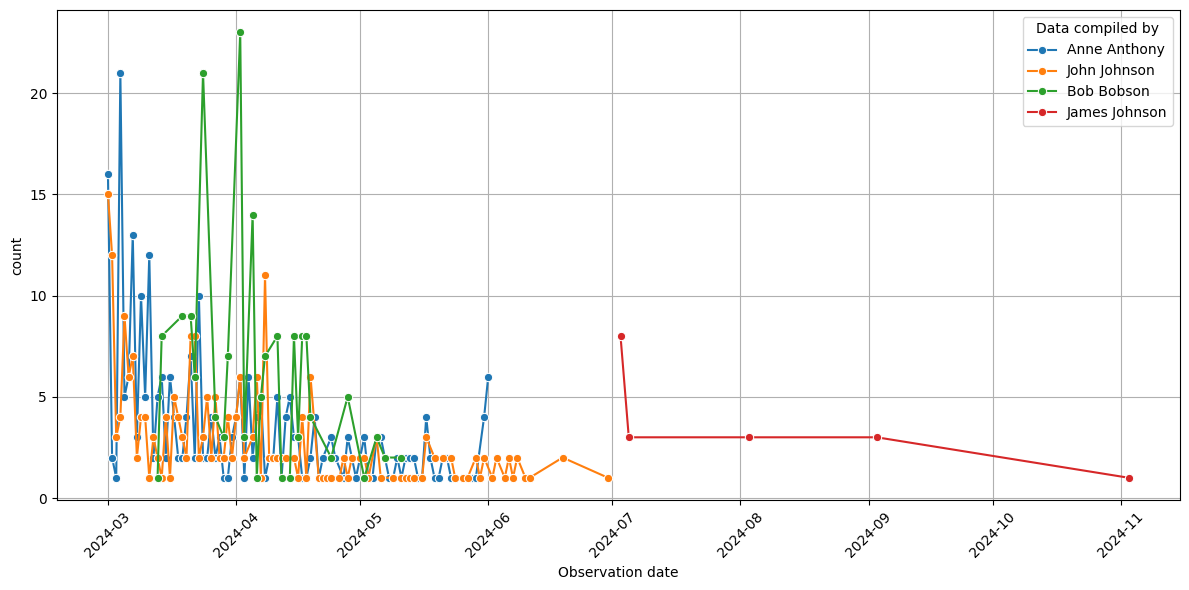
\includegraphics[width=0.8\textwidth]{images/obsdateconpiled.png}
  \caption{Line plots of observation date by gender and by data contibutor}
  \label{fig:fig3}
\end{figure}

Rivising \ref{fig:fig3}:
\begin{enumerate}
  \item All data impliments in 2024.
  \item James somewhat stanging out even more.
\end{enumerate}

\subsection{Hist and box plots}

\begin{figure}[H]
  \centering
  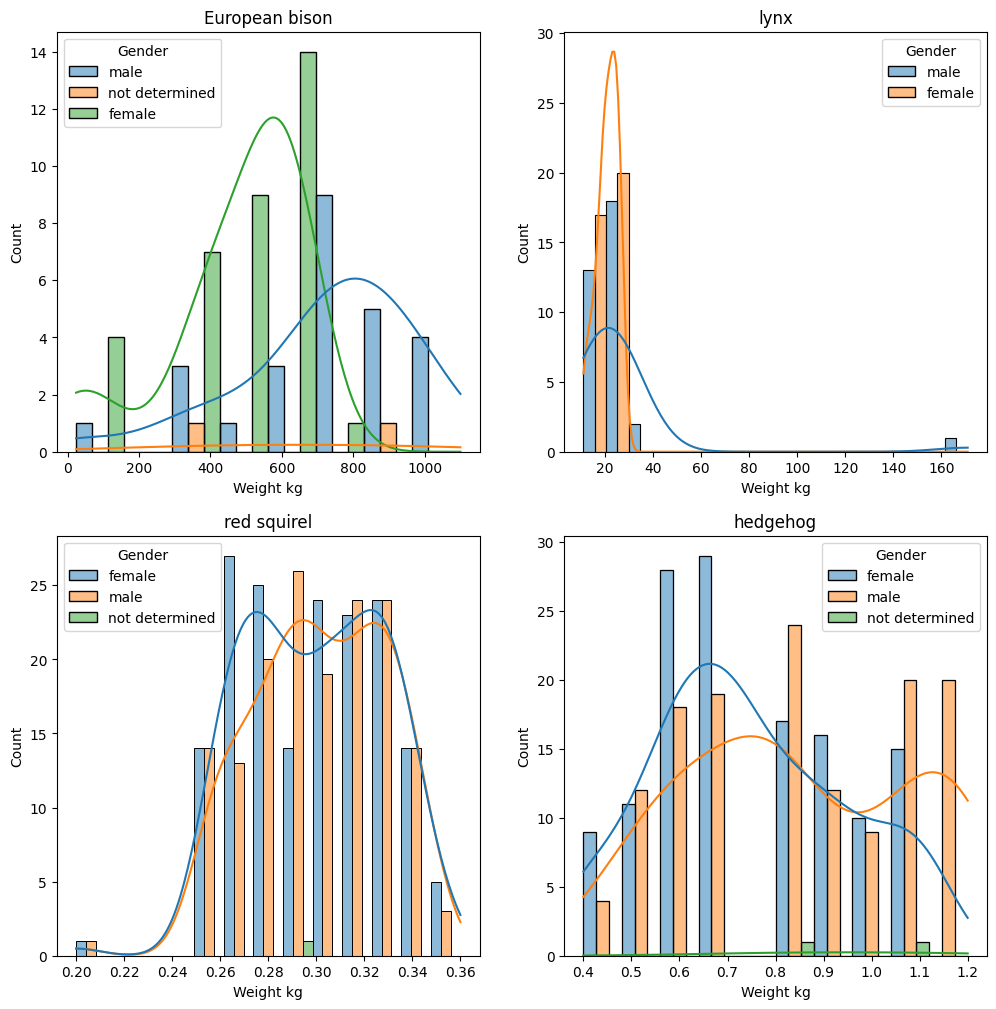
\includegraphics[width=\textwidth]{images/histweight.png}
  \caption{Distribution of weight by animal type}
  \label{fig:fig4}
\end{figure}

On~\ref{fig:fig4} nothing special except a very heavy lynx. 
No. A VERY VERY \textbf{heavy} one.

\begin{figure}[H]
  \centering
  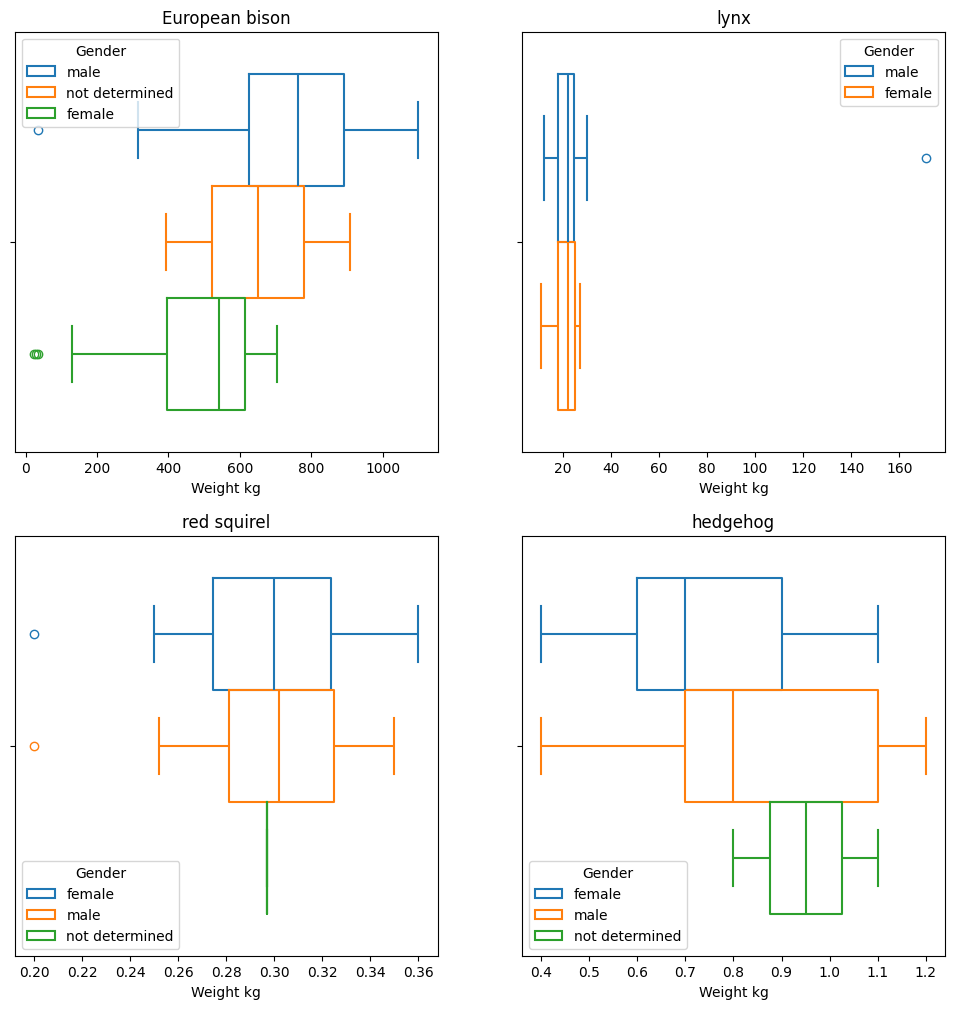
\includegraphics[width=\textwidth]{images/boxweight.png}
  \caption{Bot plots of weight by animal type}
  \label{fig:fig5}
\end{figure}

Here(\ref{fig:fig5}) the same lynx shine bright.

\begin{figure}[H]
  \centering
  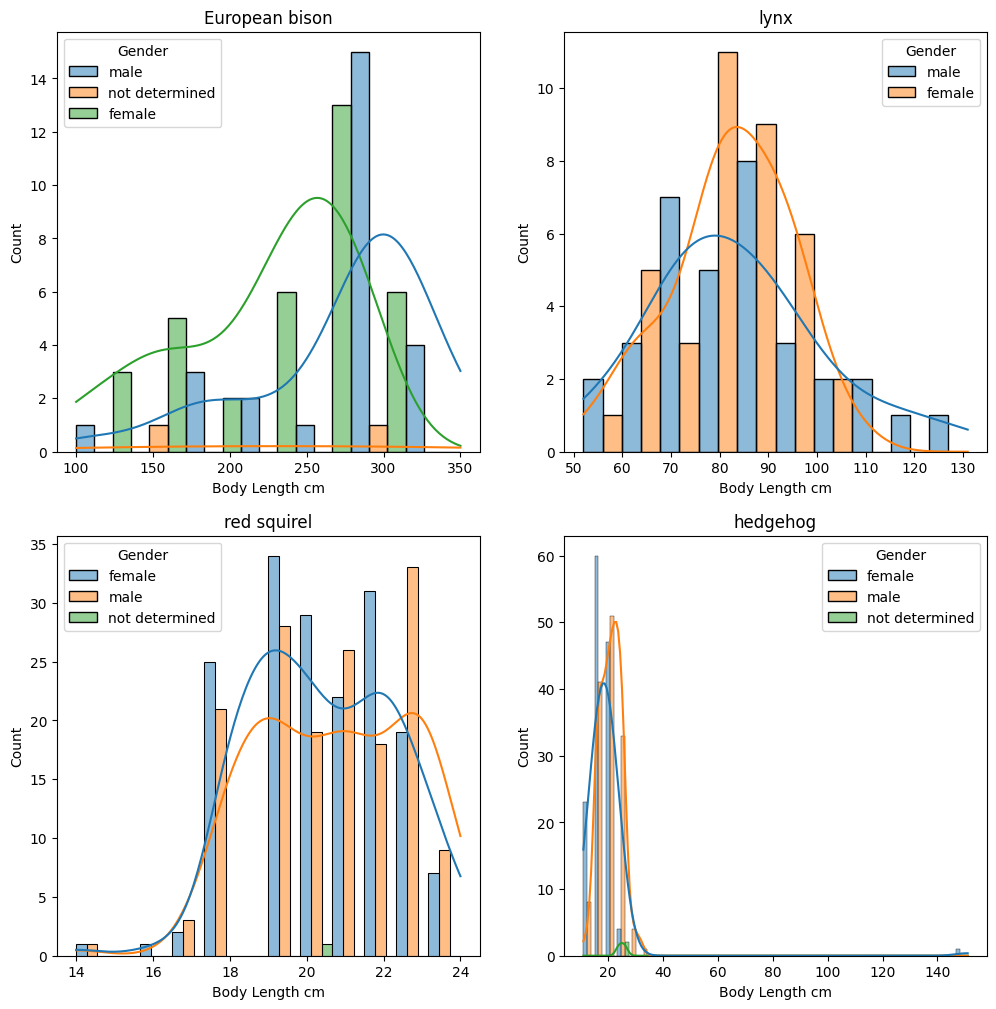
\includegraphics[width=\textwidth]{images/histlength.png}
  \caption{Distribution of lenght by animal type}
  \label{fig:fig6}
\end{figure}

As~\ref{fig:fig4} on~\ref{fig:fig6} I notice mutative animal.
Not lynx, but a new gigantic hedgehogs 150 cm long. What a monsters...
I guess it a new spicies bred by creazy Russian scientists.

\begin{figure}[H]
  \centering
  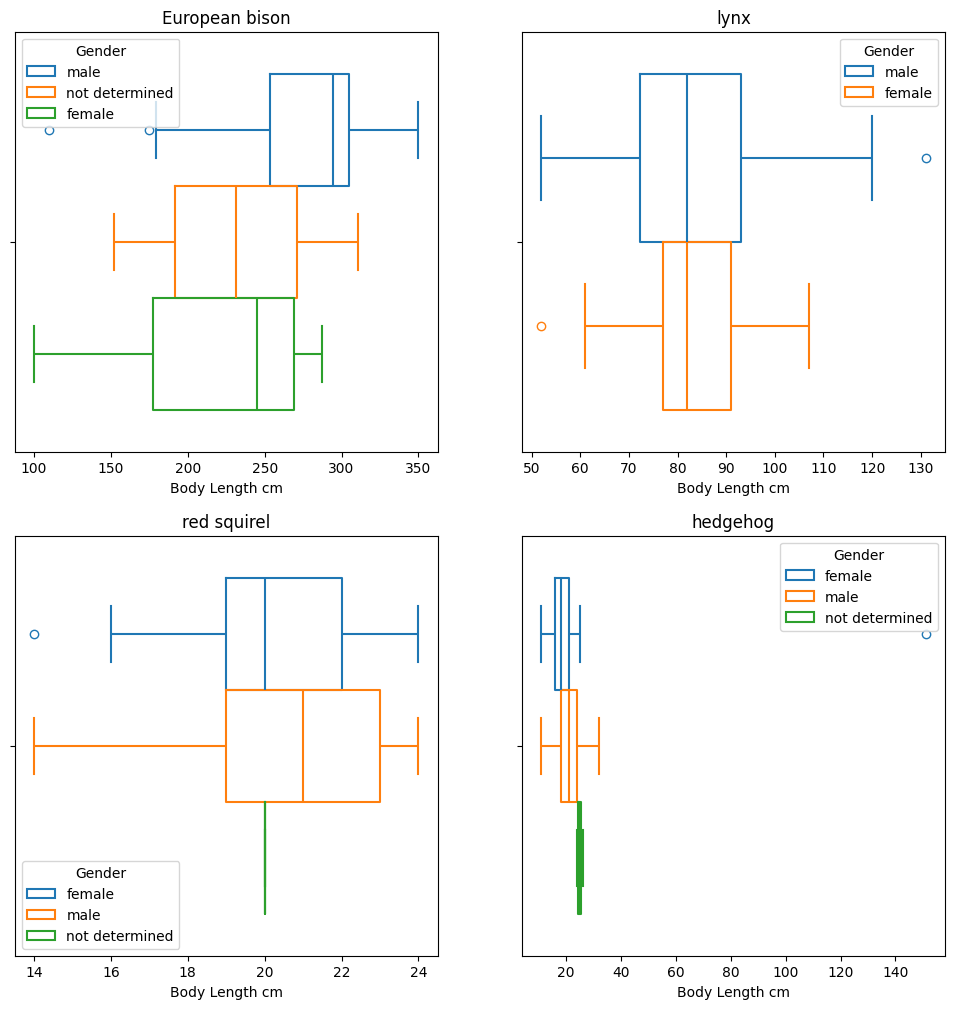
\includegraphics[width=\textwidth]{images/boxlength.png}
  \caption{Bot plots of lenght by animal type}
  \label{fig:fig7}
\end{figure}

At this moment I have no idea why I must use box plots.
They're the same as hist plots or even less intuitive.

\subsection{Pair plot}

\begin{figure}[H]
  \centering
  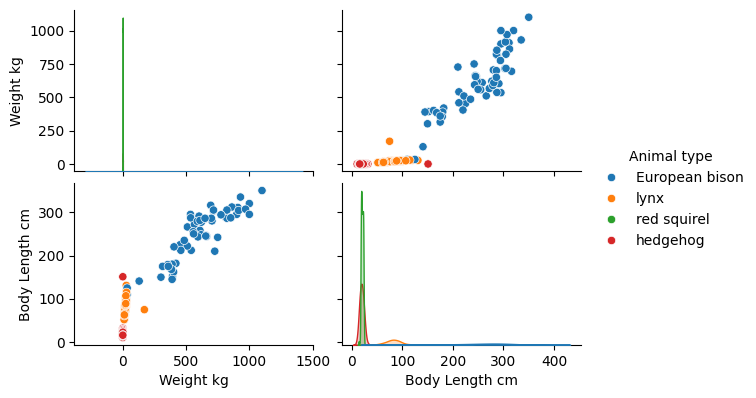
\includegraphics[width=\textwidth]{images/pairplot.png}
  \caption{Pair plot of lenght and weight}
  \label{fig:fig8}
\end{figure}

Dataset contains 4 decimal parametrs:

\begin{enumerate}
  \item Weight (kg)
  \item Lenght (kg)
  \item Latitude
  \item Longitude
\end{enumerate}

I create a pairplot of only two weight and lenghtas most interesting.
It rudiment to weight to lenght \textit{"simple"} plot.
Let's see it too:

\begin{figure}[H]
  \centering
  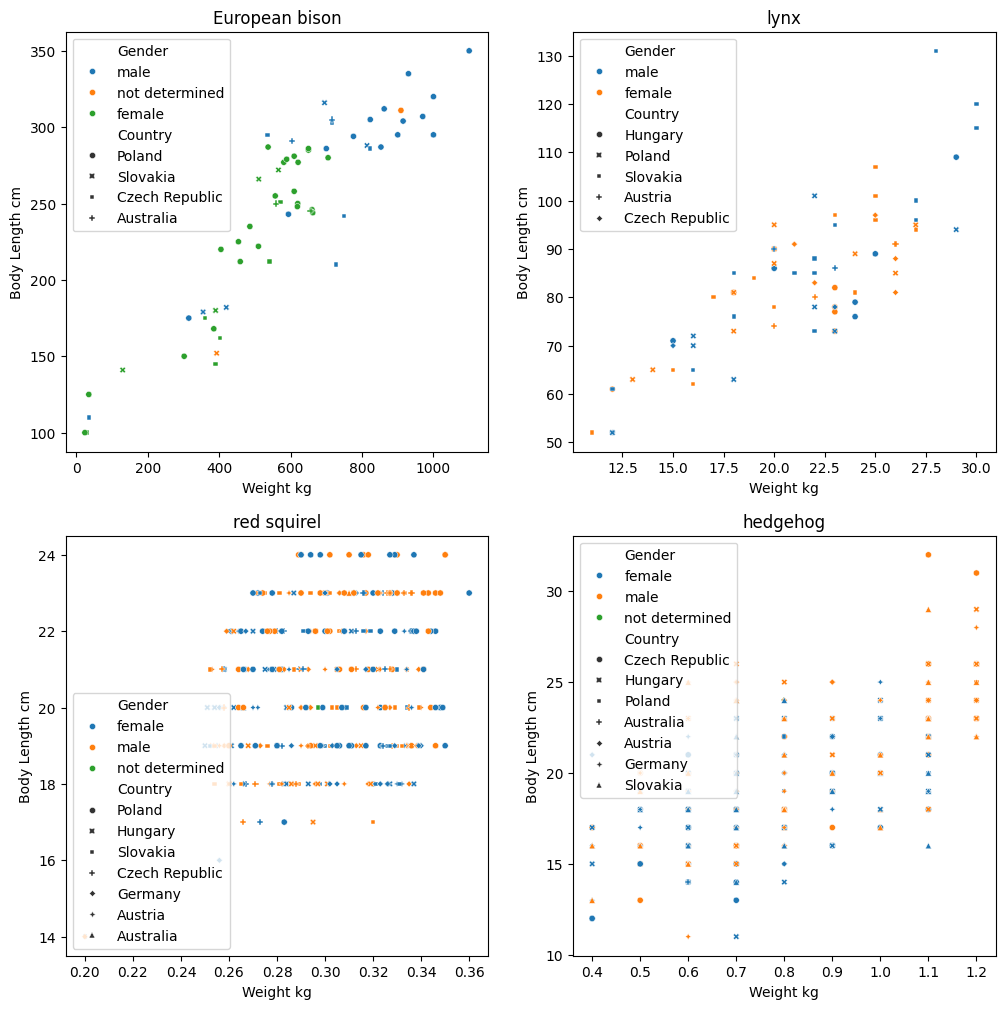
\includegraphics[width=\textwidth]{images/pairplotconsequince.png}
  \caption{Scatter plot of lenght and weight}
  \label{fig:fig9}
\end{figure}

We can see some correlation, but I cannot say anything
before I'd see correlation coefficients.

\subsection{Geo-visualization}

\begin{figure}[H]
  \centering
  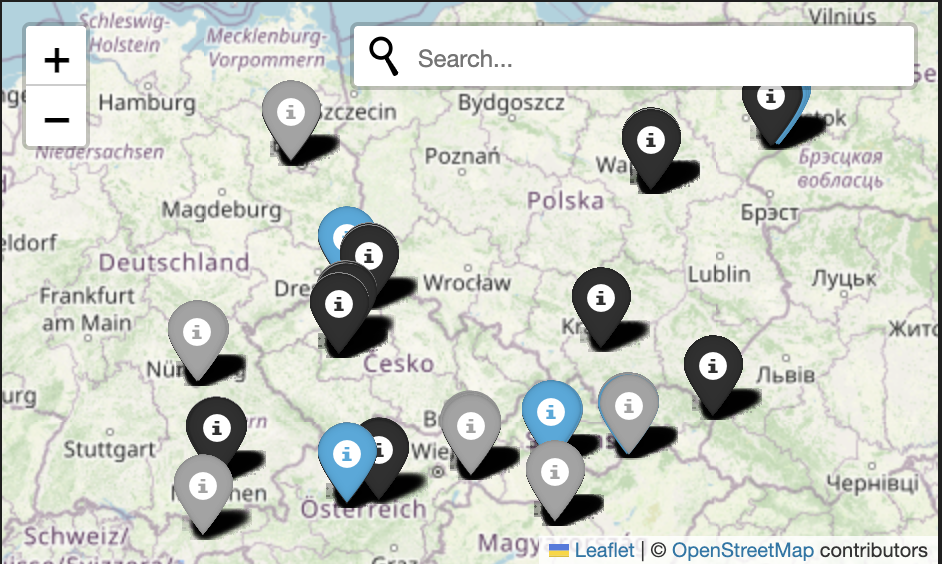
\includegraphics[width=\textwidth]{images/image.png}
  \caption{Data scattering}
  \label{fig:fig10}
\end{figure}

In this section, I want somehow visualize 2 more columns
from dataset. Here some clever way of geo-visualization.

\newpage

\section{Statistical analysis}

First of all, I used \textit{pandas.DataFrame.describe()}
option to view min, mean, max and quartiles of \textbf{wrecked data}.

\begin{table}[h]
\centering
\begin{tabular}{lrrrrr}
\hline
Statistic & Weight (kg) & Body Length (cm) & Animal code & Latitude & Longitude \\
\hline
count & 984.000000 & 984.000000 & 0.0 & 913.000000 & 913.000000 \\
mean  & 39.745503  & 39.107724  & NaN & 49.393369  & 18.203280  \\
std   & 156.290076 & 58.628601  & NaN & 7.168900   & 3.899601   \\
min   & -0.252000  & -19.000000 & NaN & -78.582973 & 11.074008  \\
25\%  & 0.293000   & 19.000000  & NaN & 48.186913  & 14.384559  \\
50\%  & 0.331500   & 21.000000  & NaN & 49.560723  & 18.944015  \\
75\%  & 0.800000   & 23.000000  & NaN & 52.212433  & 21.033243  \\
max   & 1100.000000 & 350.000000 & NaN & 52.853843  & 34.896734 \\
\hline
\end{tabular}
\caption{Descriptive statistics for \textbf{wrecked data}}
\end{table}

Right now I greatly sorrow, that I'd thought of chosing~\cite{data_link}. It was a great mistake.

Hence of this, in this section if I didn't tell another,
I used \textbf{cleaned data} in order of
simplicity. It look like this:

\begin{table}[h]
\centering
\begin{tabular}{lrrrr}
\hline
Statistic & Weight (kg) & Body length (cm) & Latitude & Longitude \\
\hline
count & 833.000000 & 833.000000 & 750.000000 & 750.000000 \\
mean  & 46.720602  & 42.501043  & 49.743041  & 17.595264  \\
std   & 168.843218 & 62.879887  & 1.851982   & 3.881169   \\
min   & 0.200000   & 11.000000  & 47.316383  & 11.074008  \\
25\%  & 0.297367   & 19.000000  & 48.186430  & 14.348471  \\
50\%  & 0.349000   & 21.000000  & 49.545885  & 18.847488  \\
75\%  & 1.000000   & 23.000000  & 52.211980  & 21.031909  \\
max   & 1100.000000 & 350.000000 & 52.853843  & 23.919668  \\
\hline
\end{tabular}
\caption{Descriptive statistics for \textbf{cleaned data}}
\end{table}

\subsection{Correlation}

Below~\ref{fig:fig11} I pin correlation maps. On this 
I can notice very strong normal correlation between weight
and lenght. Also Kendall correlation didn't show anithing.
It's strange. Let's try view correlation on diffetent
animal types.

\begin{figure}[H]
  \centering
  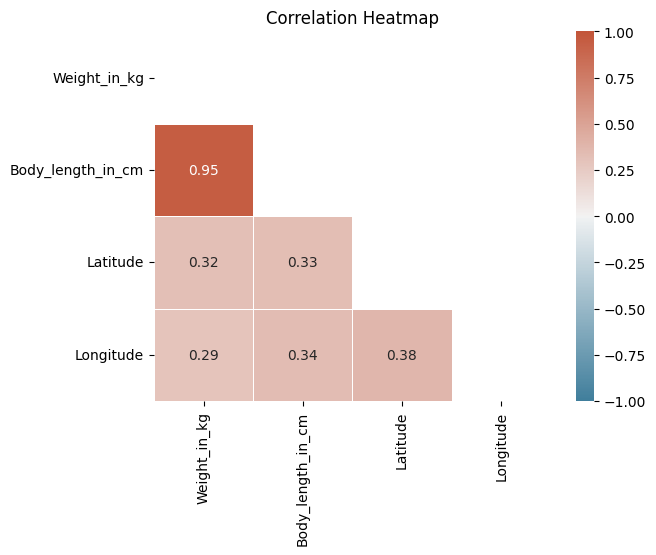
\includegraphics[width=0.9\textwidth]{images/corrheatmap.png}
  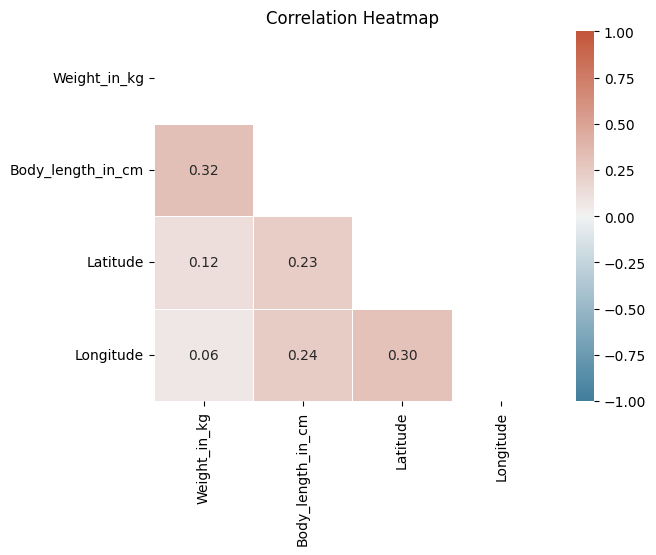
\includegraphics[width=0.9\textwidth]{images/corrheatmap2.png}
  \caption{Normal and Kendall correlation}
  \label{fig:fig11}
\end{figure}

\begin{figure}[H]
  \centering
  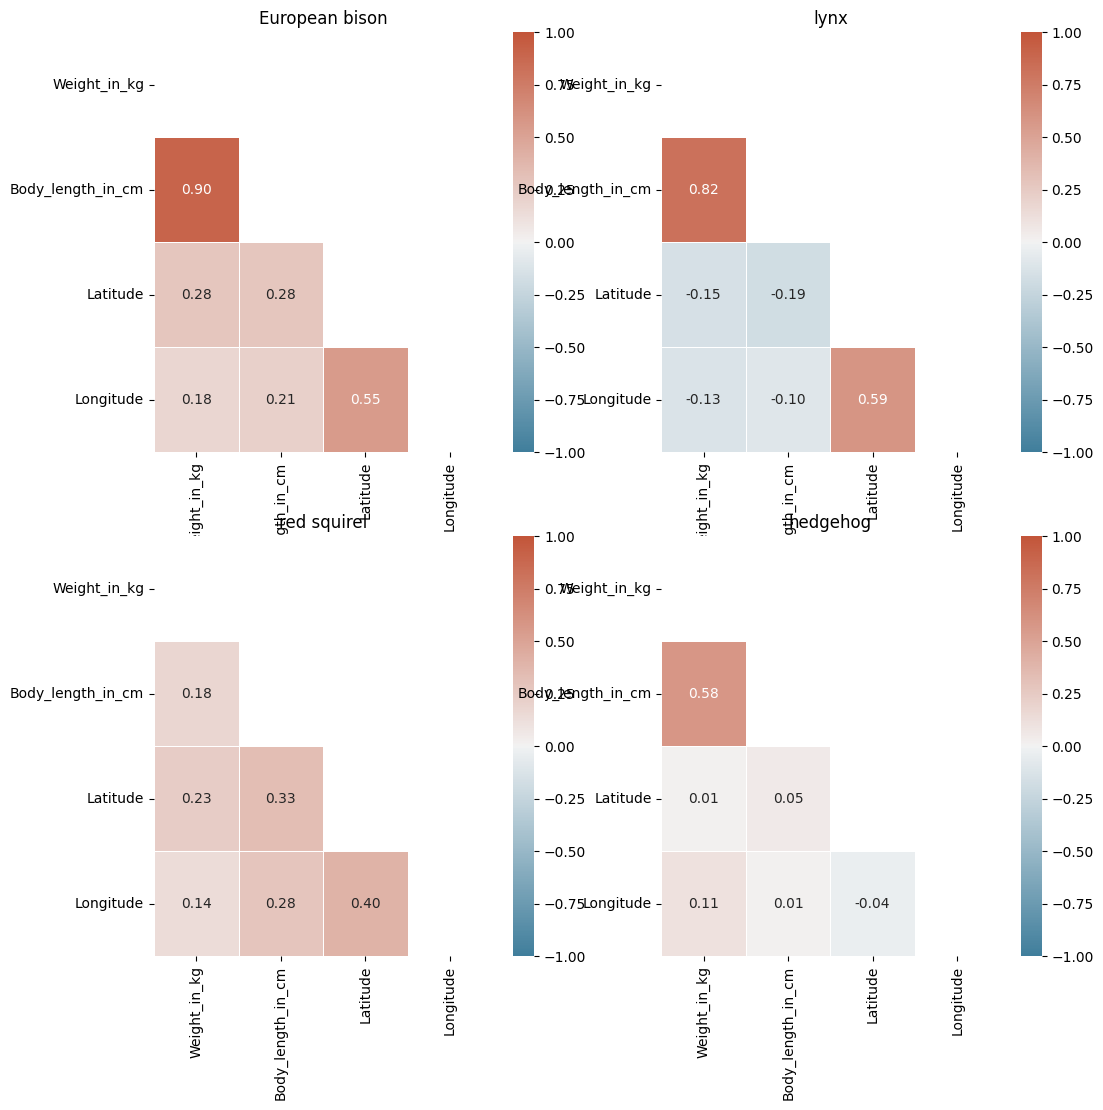
\includegraphics[width=0.75\textwidth]{images/pairheatmap.png}
  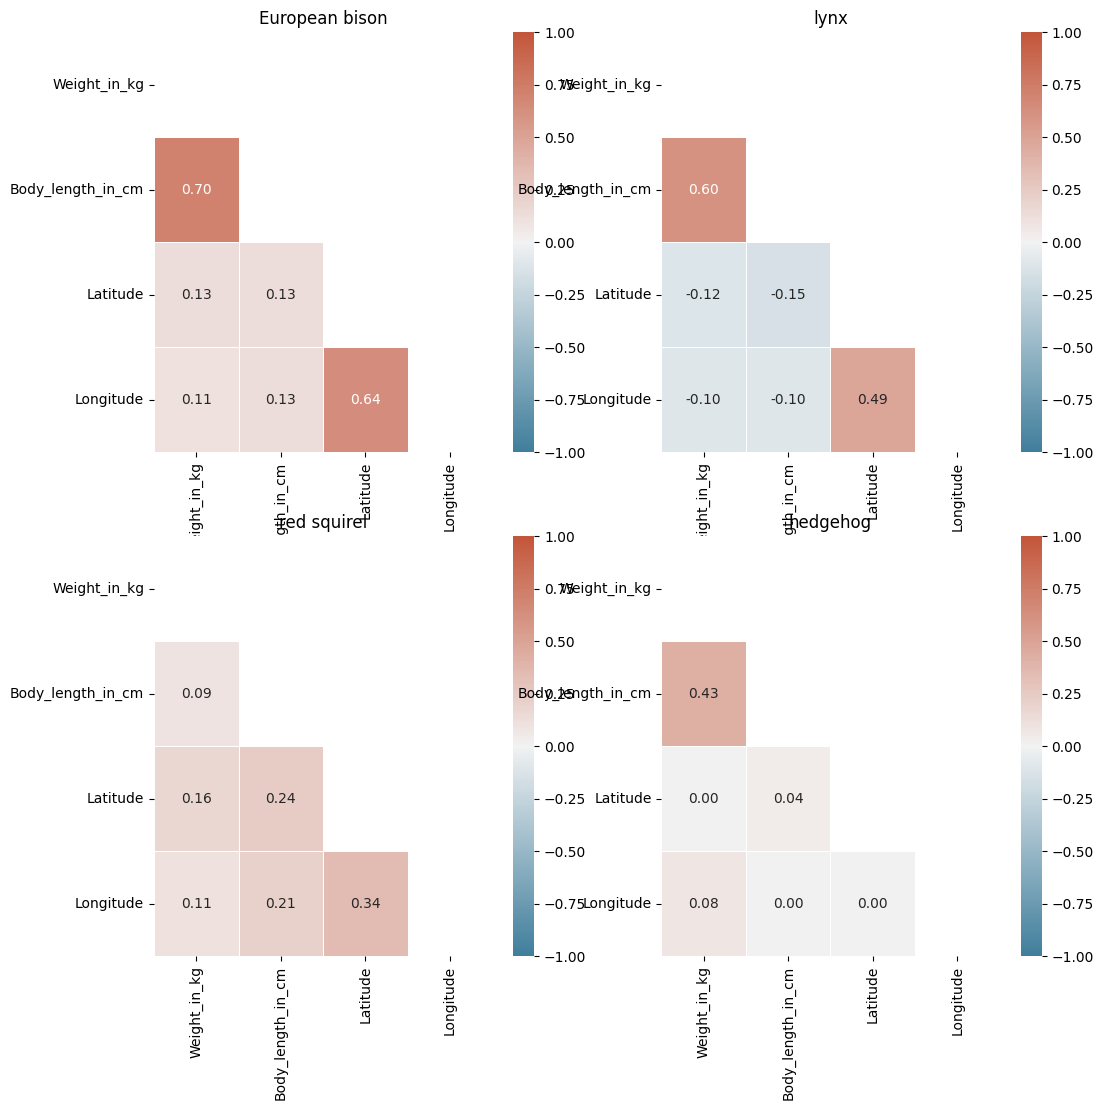
\includegraphics[width=0.75\textwidth]{images/pairheatmap2.png}
  \caption{Normal and Kendall correlation}
  \label{fig:fig12}
\end{figure}

On~\ref{fig:fig12} 4 normal correlation heat maps
and 4 Kendall correlation maps. As I can notice
This data is more optimistic. However 
$$ E[Bison(kg)] = 0.9 * E[Bison(cm)] $$
feels as well strange.
Although, as expected, latitude and longitude didn't
correlate with anithing much.
Let's move on with this wonderful quote:

\textit{"Correlation does not imply causation" }

\subsection{Is lynx? lynx?}

When I wrote \textit{dirty\_data["Animal\_type"].unique()}, I discovered class lynx?:
\begin{verbatim}
array([nan, 'European bison', 'European bison™', 'European bisson',
       'European buster', 'lynx', 'lynx?', 'red squirel', 'red squirrel',
       'red squirrell', 'hedgehog', 'wedgehod', 'ledgehod'], dtype=object)
\end{verbatim}
I found question \textit{"Is lynx? lynx?"} interesting to me.
Let's find it out!

First of all I tryed to use t-values:
\begin{enumerate}
  \item For \textbf{body length in cm}: $$t-statistic: -0.5793803445653539, p-value: 0.5642194350169902$$
  \item For \textbf{weight in kg}: $$t-statistic: 0.28872058707288334, p-value: 0.7736608274782608$$
\end{enumerate}
For both cases $p-value >> 0.05$, this mean significant differences in classes. 
I'd already lost trast in statistic\dots

\begin{thebibliography}{99}
\bibitem{data_link} \href{https://www.kaggle.com/datasets/joannanplkrk/dirty-data-to-clean-whats-wrong-with-this-dataset}{Dirty data to clean What's wrong with this dataset}.
\end{thebibliography}

\end{document} % End of document
